\section{The Model DNABERT}

DNABERT is a model that follows the same paradigms introduced by BERT, but adapted to the DNA sequences \cite{DBLP:journals/corr/abs-1810-04805}.
BERT is a transformer-based contextualized language representation model that has achieved superhuman performance in many natural language processing (NLP) tasks. It introduces a paradigm of pre-training and fine-tuning, which first develops general-purpose understandings from massive amount of unlabeled data and then solves various applications with task-specific data with minimal architectural modification.


\subsection{Architecture}

The DNABERT model adopts the same architecture as BERT-base:
\begin{itemize}
    \item 12 Transformer encoder layers
    \item 768-dimensional hidden states
    \item 12 self-attention heads
\end{itemize} 

Each input sequence is limited to a maximum of 512 tokens and is enclosed between two special tokens: [CLS] and [SEP]. As in the original BERT, the [CLS] token is used to represent the entire input sequence and is utilized for sequence-level predictions such as classification tasks.

However, unlike standard BERT, DNABERT is specifically adapted to the genomic domain through a different tokenization scheme. Instead of using WordPiece, it tokenizes DNA sequences using k-mers, where each k-mer is a substring of length k (with k = 3, 4, 5, or 6). This strategy captures richer local nucleotide context and reduces sparsity. For each value of k, a separate DNABERT model is trained (e.g., DNABERT-3, DNABERT-4, etc.).

The input to DNABERT is thus a sequence of overlapping k-mers, converted to embeddings through the sum of three vectors:
\begin{itemize}
    \item Token embeddings (for each k-mer),
    \item Position embeddings (to encode sequence order),
    \item Segment embeddings (to distinguish sequence segments, although only one segment is typically used for DNA).
\end{itemize}

Internally, the model applies standard Transformer operations: multi-head self-attention, feed-forward layers, residual connections, and layer normalization—repeated across all 12 layers, as shown in the \autoref{fig:dnabert-arch}.

\begin{figure}[h!]
    \centering
    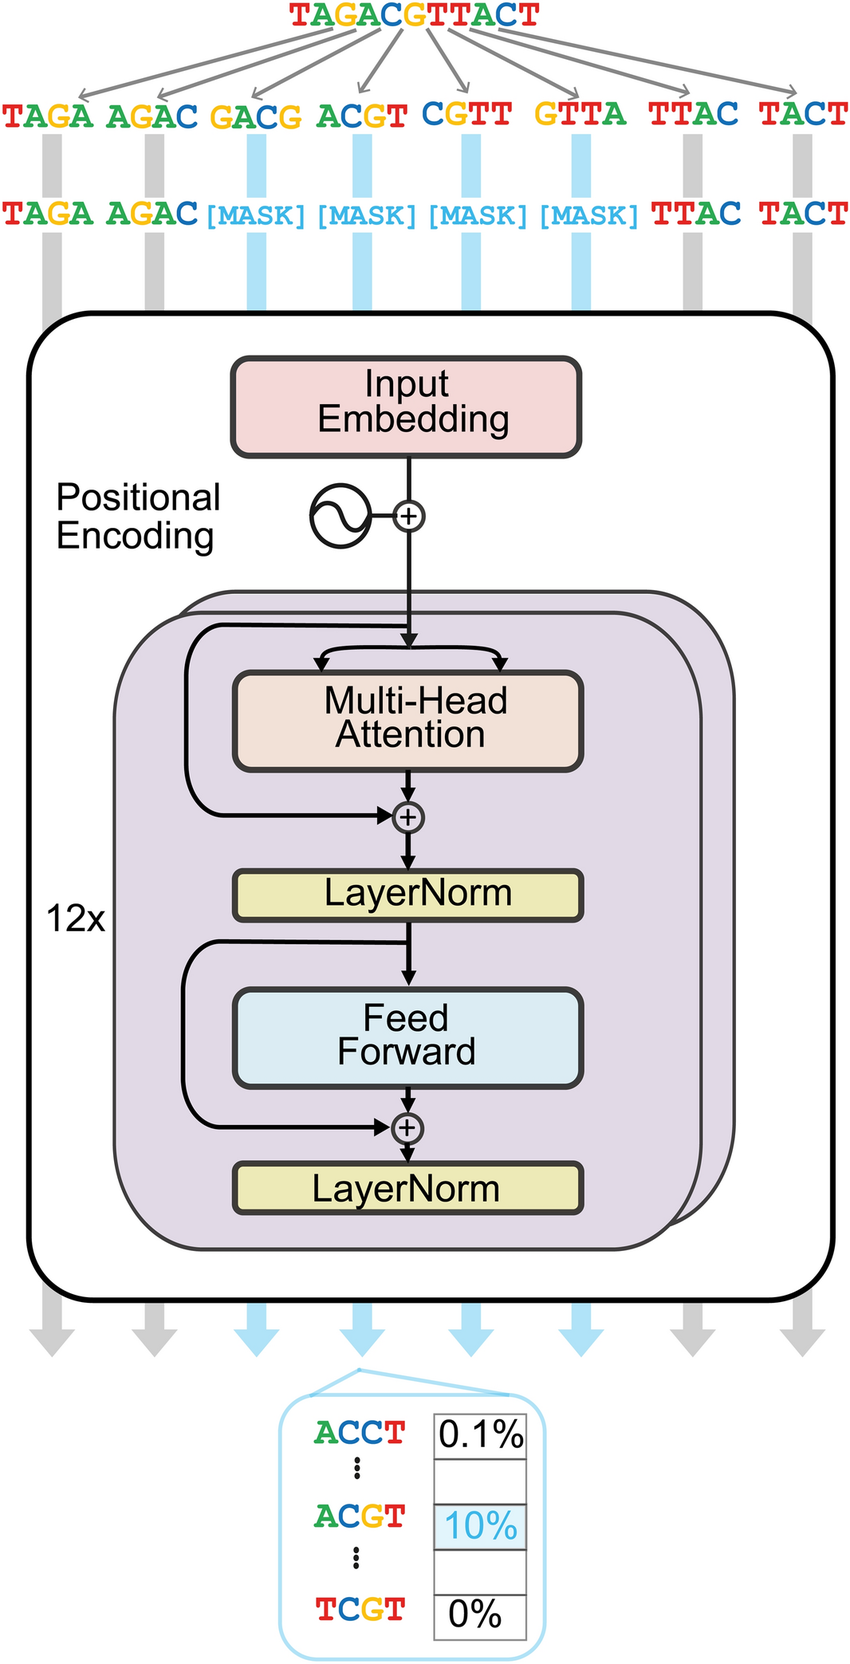
\includegraphics[width=.6\linewidth]{imgs/model-arch.png}
    \caption{The model architecture of DNABERT \cite{384017589}}
    \label{fig:dnabert-arch}
\end{figure}

During pre-training, DNABERT uses a masked language modeling (MLM) objective, like BERT, but without next sentence prediction (NSP), which is not applicable in genomic contexts. Approximately 15–20\% of k-mers in each sequence are randomly masked in contiguous spans, and the model is trained to predict them based on surrounding context. This enables the model to learn the "syntax" and "semantics" of genomic sequences in a self-supervised fashion.

To support sequences longer than 512 tokens, DNABERT also provides an extended version called DNABERT-XL, where long sequences are split into chunks, independently processed, and their representations concatenated.

\subsection{Pretraining}

The pretraining of DNABERT is performed in a self-supervised fashion, meaning that no labeled data is required. Similar to the original BERT, DNABERT uses a Masked Language Modeling (MLM) objective: approximately 15\% to 20\% of the input k-mer tokens are randomly masked, and the model is trained to predict these masked tokens based on the surrounding context.

Unlike the original BERT, where individual tokens are masked, DNABERT masks contiguous spans of k-mers. This is crucial because individual k-mers can often be trivially inferred from adjacent ones due to overlapping, especially in genomic sequences. Masking contiguous regions prevents the model from "cheating" and encourages it to learn deeper contextual relationships across upstream and downstream nucleotide patterns.

The goal of pretraining is to allow DNABERT to learn general-purpose representations of DNA, capturing both local motifs and long-range dependencies, without requiring any manual annotations. The learned embeddings encode the "syntax" and "semantics" of non-coding DNA regions, enabling effective transfer to various downstream tasks such as promoter prediction, transcription factor binding site (TFBS) identification, and splice site detection.

DNABERT was pretrained on the entire human genome, using input sequences of varying lengths (from 10 to 510 k-mers), sampled via both random and non-overlapping segmentation strategies. The model was trained for 120,000 steps with a batch size of 2000. During the first 100,000 steps, a masking rate of 15\% was used, which was increased to 20\% in the final 20,000 steps. The learning rate followed a warm-up and linear decay schedule, peaking at 4e-4. 

Pretraining was computationally intensive, taking approximately 25 days on 8 NVIDIA 2080Ti GPUs. Four separate models were trained, corresponding to different k-mer granularities: k = 3, 4, 5, and 6. Among these, DNABERT-6 (with 6-mers) achieved the best performance and was used in the majority of downstream experiments.

This extensive pretraining enables DNABERT to serve as a general foundation model for genomic sequence analysis, capable of achieving strong performance even in data-scarce settings.

\subsection{Fine-tuning}

Once pretrained, DNABERT can be easily fine-tuned on a variety of downstream genomic tasks by adding a lightweight task-specific classification head on top of the [CLS] token output and continuing training on a small labeled dataset. This transfer learning approach allows the model to adapt its general understanding of DNA sequence patterns to more specific biological functions with minimal additional supervision.

DNABERT has been successfully fine-tuned for several key tasks in regulatory genomics, including:
\begin{itemize}
    \item Promoter prediction: identifying proximal and core promoter regions around transcription start sites (TSS), including both TATA and non-TATA promoters.

    \item Splice site recognition: detecting canonical and non-canonical donor and acceptor sites, even in the presence of confounding sequence motifs.

    \item Transcription factor binding site (TFBS) identification: locating precise DNA segments bound by transcription factors, using ChIP-seq enriched regions.
\end{itemize}

During fine-tuning, the pretrained weights of DNABERT are updated jointly with the classifier head using task-specific data. The training typically employs optimization strategies such as learning rate warm-up, linear decay, dropout regularization, and the AdamW optimizer. Hyperparameters are tuned on a validation set to maximize generalization.

A key strength of DNABERT lies in its ability to achieve state-of-the-art performance even with limited labeled data, thanks to the rich representations learned during pretraining. Additionally, the model generalizes well across species: for instance, a DNABERT model pretrained on the human genome was effectively fine-tuned on mouse transcription factor datasets, demonstrating strong cross-organism transfer capabilities.

\subsection{Advantages}

DNABERT introduces three key advantages over previous models such as CNNs and RNNs:
\begin{itemize}
    \item It captures long-range dependencies through a global attention mechanism.
    \item It generalizes well across multiple tasks.
    \item It requires only a small amount of labeled data for fine-tuning.
\end{itemize}

Additionally, the model’s architecture allows for an intuitive interpretation of biological signals through attention maps.